\documentclass[aspectratio=169]{beamer}

\usepackage{ccicons}
\usepackage{fontspec}
\usepackage{listings}
\usepackage{tikz}
\usepackage{svg}

\definecolor{uclablue}{RGB}{39,116,174}
\definecolor{uclagold}{RGB}{255,179,0}

\definecolor{ubcorange}{RGB}{158, 66, 37}

\definecolor{cugold}{RGB}{207, 184, 124}
\definecolor{cudarkgray}{RGB}{86, 90, 92}

\definecolor{solarizedred}{RGB}{220, 50, 47}
\definecolor{solarizedblue}{RGB}{38, 139, 210}
\definecolor{solarizedgreen}{RGB}{133, 153, 0}
\definecolor{solarizedpurple}{RGB}{108, 113, 196}
\definecolor{solarizedmagenta}{RGB}{211, 54, 130}

\definecolor{pantone655}{RGB}{0, 42, 92}
\definecolor{pantone7453}{RGB}{123, 164, 217}
\definecolor{pantone633}{RGB}{0, 139, 176}
\definecolor{pantone7492}{RGB}{218, 229, 205}

\colorlet{primarycolor}{pantone655}
\colorlet{secondarycolor}{pantone7453}


\usetikzlibrary{
  arrows,
  arrows.meta,
  automata,
  backgrounds,
  calc,
  chains,
  decorations.pathreplacing,
  fit,
  intersections,
  matrix,
  overlay-beamer-styles,
  positioning,
  shapes,
  shapes.multipart,
  tikzmark,
}
\usetikzmarklibrary{listings}

\hypersetup{
  colorlinks=true,
  urlcolor=cudarkgray,
}

\setbeamercolor{frametitle}{fg=primarycolor}
\setbeamercolor{structure}{fg=primarycolor}
\setbeamercolor{enumerate item}{fg=black}
\setbeamercolor{itemize item}{fg=black}
\setbeamercolor{itemize subitem}{fg=black}

\setbeamersize{text margin left=26.6mm}
\addtolength{\headsep}{2mm}

\setbeamertemplate{navigation symbols}{}
\setbeamertemplate{headline}{}
\setbeamertemplate{footline}{}
\setbeamertemplate{itemize item}{\color{black}}
\setbeamertemplate{itemize items}[circle]

\setbeamertemplate{footline}{
  \begin{tikzpicture}[remember picture,
                      overlay,
                      shift={(current page.south west)}]
    \node [black!50, inner sep=2mm, anchor=south east]
          at (current page.south east) {\footnotesize \insertframenumber};
  \end{tikzpicture}
}

\setsansfont{Inter}[Scale=MatchLowercase]
\setmonofont{Hack}[Scale=MatchLowercase]

\makeatletter
\newcommand\version[1]{\renewcommand\@version{#1}}
\newcommand\@version{}
\def\insertversion{\@version}

\newcommand\lecturenumber[1]{\renewcommand\@lecturenumber{#1}}
\newcommand\@lecturenumber{}
\def\insertlecturenumber{\@lecturenumber}
\makeatother

\setbeamertemplate{title page}
{
  \begin{tikzpicture}[remember picture,
                      overlay,
                      shift={(current page.south west)},
                      background rectangle/.style={fill=pantone655},
                      show background rectangle]
    \node [anchor=west, align=left, inner sep=0, text=white]
          (lecturenumber) at (\paperwidth / 6, \paperheight * 3 / 4)
          {\Large Lecture \insertlecturenumber};
    \node [inner sep=0, align=left, text=white, node distance=0,
          above left=of lecturenumber, anchor=south west, yshift=2mm]
          {\Large ECE 344: Operating Systems};
    \node (title) [inner sep=0, anchor=west, align=left, text=white,
                   text width=30em]
          at (\paperwidth / 6, \paperheight / 2)
          {{\bfseries \Huge \inserttitle{}}};
    \node [inner sep=0, align=right, text=white, node distance=0,
          below right=of title, anchor=north east, yshift=-1mm]
          {{\footnotesize \ttfamily \insertversion}};
    \node [inner sep=0, text=white, align=left, anchor=west]
          (author) at (\paperwidth / 6, \paperheight / 4)
          {\insertauthor};
    \node [text=white, inner sep=0, align=left, node distance=0,
           below left=of author, anchor=north west, yshift=-2mm]
          {\insertdate};
    \node [align=right, anchor=south east, inner sep=2mm, text=white]
          (license) at (\paperwidth, 0)
          {\footnotesize This  work is licensed under a
           \href{http://creativecommons.org/licenses/by-sa/4.0/}
                {\color{pantone7453} Creative Commons Attribution-ShareAlike 4.0
                 International License}};
    \node [text=white, inner sep=0, align=right, node distance=0,
           above right=of license, anchor=south east, xshift=-2mm]
          {\Large \ccbysa};
  \end{tikzpicture}
}

\tikzset{
  >=Straight Barb[],
  shorten >=1pt,
  initial text=,
}

\lstset{
  basicstyle=\footnotesize\ttfamily,
  language=C,
  escapechar=@,
  commentstyle=\color{black!50},
}


\lecturenumber{4}
\title{Process Creation}
\version{1.0.0}
\author{Jon Eyolfson}
\date{September 15, 2022}

\begin{document}
  \begin{frame}[plain, noframenumbering]
    \titlepage
  \end{frame}

  \begin{frame}
    \frametitle{We Could Create Processes from Scratch}

    We load the program into memory and create the process control block

    \vspace{2em}

    This is what Windows does

    \vspace{4em}

    Unix decomposes process creation into more flexible abstractions
  \end{frame}

  \begin{frame}
    \frametitle{Instead of Creating a New Process, We Could Clone It}

    Pause the currently running process, and copy it's PCB into a new one

    \hspace{2em} This will reuse all of the information from the process,
    including variables!

    \vspace{2em}

    Distinguish between the two processes with a parent and child relationship

    \hspace{2em} They could both execute different parts of the program together

    \vspace{4em}

    We could then allow either process to load a new program and setup a new PCB
  \end{frame}

  \begin{frame}
    \frametitle{A Typical Process Tree on the Virtual Machine}

    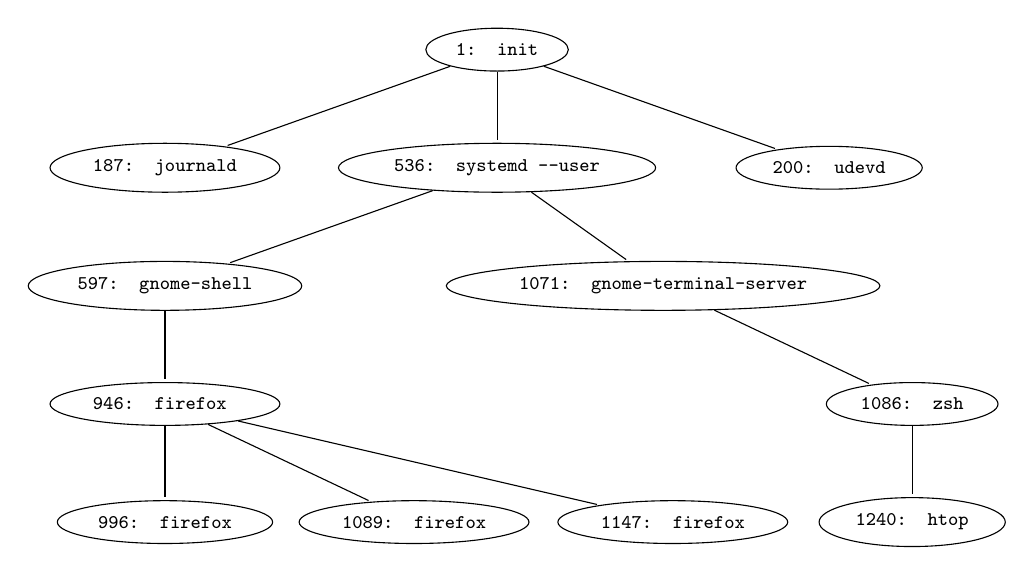
\begin{tikzpicture}[sibling distance=12em]
      \tikzstyle{every node}=[ellipse, draw, font=\scriptsize\ttfamily, align=center]
      \node {1: init}
        child { node {187: journald} }
        child { node {536: systemd --user}
          child { node [xshift=-6em] {597: gnome-shell}
            child { node { 946: firefox }
              child { node [xshift=12em] {996: firefox} }
              child { node [xshift=9em] {1089: firefox} }
              child { node [xshift=6.35em] {1147: firefox} }
            }
          }
          child { node {1071: gnome-terminal-server}
            child { node [xshift=9em] {1086: zsh}
              child { node {1240: htop}
              }
            }
          }
        }
        child { node {200: udevd} };
    \end{tikzpicture}
  \end{frame}

  \begin{frame}
    \frametitle{How You Can See Your Process Tree}

    Use \texttt{htop}

    \vspace{2em}

    You can press \texttt{F5} to switch between tree and list view
  \end{frame}

  \begin{frame}
    \frametitle{Linux Terminology Is Slightly Different}

    You can look at a process' state by reading \texttt{/proc/<PID>/status | grep State}

    \hspace{2em} Replace \texttt{<PID>} with the process ID (or \texttt{self})

    \vspace{2em}

    R: Running and runnable [Running and Waiting]

    S: Interruptible sleep [Blocked]

    D: Uninterruptible sleep [Blocked]

    T: Stopped

    Z: Zombie

    \vspace{2em}

    The kernel lets you explicitly stop a process to prevent it from running

    \hspace{2em} You or another process must explicitly continue it
  \end{frame}

  \begin{frame}
    \frametitle{On Unix, the Kernel Launches A Single User Process}

    After the kernel initializes, it creates a single process
    from a program

    \vspace{2em}

    This process is called \texttt{init}, and it looks for it in \texttt{/sbin/init}

    \hspace{2em} Responsible for executing every other process on the machine

    \hspace{2em} Must always be active, if it exits the kernel thinks you're shutting down

    \vspace{2em}

    For Linux, \texttt{init} will probably be \texttt{systemd} but there's other options

    \vspace{2em}

    Aside: some operating systems create an ``idle'' process that the
    scheduler can run
  \end{frame}

  \begin{frame}
    \frametitle{Standard File Descriptors for Unix}

    All command line executables use the following standard for file
    descriptors:

    \begin{itemize}
      \item \texttt{0} --- \texttt{stdin} (Standard input)
      \item \texttt{1} --- \texttt{stdout} (Standard output)
      \item \texttt{2} --- \texttt{stderr} (Standard error)
    \end{itemize}

    \vspace{2em}

    The terminal emulators job is to:
    \begin{itemize}
      \item Translate key presses to bytes and write to \texttt{stdin}
      \item Display bytes read from \texttt{stdout} and \texttt{stderr}
      \item May redirect file descriptors between processes
    \end{itemize}
  \end{frame}

  \begin{frame}[fragile]
    \frametitle{Checking Open File Descriptors on Linux}

    \texttt{/proc/<PID>/fd} \hspace{0.5em} is a directory containing all open
    file descriptors for a process

    \texttt{ps x} \hspace{0.5em} command shows a list of processes matching your
    user (lots of other flags)

    \vspace{1em}

    A terminal emulator may give the output:
    \begin{lstlisting}[basicstyle=\small\ttfamily]
> ls -l /proc/21151/fd
0 -> /dev/tty1
1 -> /dev/tty1
2 -> /dev/tty1
    \end{lstlisting}

    \vspace{2em}

    \texttt{lsof <FILE>} \hspace{0.5em} shows you what processes have the file
    open

    \hspace{2em} For example, processes using C: \hspace{0.5em}
    \texttt{lsof /lib/libc.so.6}
  \end{frame}

  \begin{frame}
    \frametitle{On POSIX Systems, You Can Find Documentation Using \texttt{man}}

    We'll be using the following APIs:
    \begin{itemize}
      \item \texttt{execve} (last lecture)
      \item \texttt{fork} (today)
      \item \texttt{wait} (next lecture)
    \end{itemize}

    \vspace{2em}

    You can use \texttt{man <function>} to look up documentation,

    or \texttt{man <number> <function>}

    \hspace{2em} 2: System calls

    \hspace{2em} 3: Library calls
  \end{frame}

  \begin{frame}
    \frametitle{\texttt{fork} Creates a New Process, A Copy of the Current One}

    \texttt{fork} as the following API:
    \begin{itemize}
      \item Returns the process ID of the newly created child process

            \hspace{2em} -1: on failure

            \hspace{2em} 0: in the child process

            \hspace{2em} >0: in the parent process
    \end{itemize}

    \vspace{2em}

    There are now 2 processes running

    \hspace{2em} Note: they can access the same variables, but they're separate

    \hspace{4em} Operating system does ``copy on write'' to maximize sharing
  \end{frame}

  \begin{frame}[fragile]
    \frametitle{\texttt{fork-example.c} Has One Process Execute Each Branch}

    \begin{lstlisting}
int main(int argc, char *argv[]) {
  pid_t pid = fork();
  if (pid == -1) {
    int err = errno;
    perror("fork failed");
    return err;
  }
  if (pid == 0) {
    printf("Child returned pid: %d\n", pid);
    printf("Child pid: %d\n", getpid());
    printf("Child parent pid: %d\n", getppid());
  }
  else {
    printf("Parent returned pid: %d\n", pid);
    printf("Parent pid: %d\n", getpid());
    printf("Parent parent pid: %d\n", getppid());
  }
  return 0;
}
    \end{lstlisting}
  \end{frame}

  \begin{frame}
    \frametitle{Unix Systems Clone Processes with a Parent/Child Relationship}

    \begin{itemize}
      \item You can only create new processes with \texttt{fork}
      \item After a \texttt{fork} both processes are exactly the same
      \begin{itemize}
        \item except for the value of \texttt{pid} (the child is always 0)
      \end{itemize}
      \item The scheduler decides when to run either process
    \end{itemize}
  \end{frame}
\end{document}
